%%% Endowing the Pisa/IIT SoftHand with the sense of touch

\subsubsection{Endowing the Pisa/IIT SoftHand with the sense of touch}
\label{sec:SenseOfTouch}

\noindent $\blacktriangleright$  \textbf{The Madgwick Filter} \\ 
\newline

The Mahony-Hamel filter showed in section \ref{MahonyHamel} is a modified version of the original one, to return in the correction term expression eq. (\ref{vex}) a complete information about errors given by accelerometer and compass measurements. However in his works Sebastian Madgwick shows a new algorithm able to better use the measures read by sensors. Algorithm proposed is also able to tackle the singularities, associated for example with Euler angle representation, using quaternions to represent a general orientation. The Madgwick filter is similar to Mahony-Hamel filter, in each time a new orientation quaternion is estimated summing to its previously estimation a correction factor, which depends by
data read from IMU.  %All quaternions used in this section are to be considered unity normalized. 

Let be ${^b\omega_x}$, ${^b\omega_y}$ and ${^b\omega_z}$ angular rate measures (in $\rad s^{-1}$) with respect the IMU body frame $\{ B \}$ respectively about $x$, $y$ and $z$ axis and $^{b}\Omega$ a vector cointaing these measures as

\begin{equation}
\label{eq4_01}
^b \Omega = [ 0 \quad {^b\omega_x} \quad {^b\omega_y} \quad {^b\omega_z} ],
\end{equation}

\noindent the quaternion describing the rate of change of the earth frame $\{ A \}$ with respect to the sensor frame $\{ B \}$ can be written as

\begin{equation}
\label{eq4_02}
^b_a\dot{q} = \frac{1}{2} {^b_a \bar{q}}  \otimes {^b\Omega}.
\end{equation}

\noindent Where $\otimes$ denotes a quaternion product, while $\bar{}$ denotes the unity normalize operator. From eq. (\ref{eq4_02}) trivially the orientation of the earth frame with respect to sensor frame at time \textit{t} is given by eq. (\ref{eq4_03}) and (\ref{eq4_04}) as

\begin{equation}
\label{eq4_03}
^b_a \dot{q}_{\Omega,t} = \frac{1}{2} {^b_a \hat{\bar{q}}_{t-1}} \otimes ^b \Omega_t,
\end{equation}

\begin{equation}
\label{eq4_04}
^b_a q_{\Omega,t} = {^b_a \hat{\bar{q}}_{t-1}} + {^b_a \dot{q}_{\Omega,t}} \Delta t,
\end{equation} 

\noindent where $^b \Omega_t$ is angular rate measured at time \textit{t}, $\Delta t$ is the sampling period and $^b_a \hat{\bar{q}}_{t-1}$ is the previous estimate of the orientation quaternion.

Reading now from a sensor a set of accelerometer and compass measures in a frame strap down to the sensor there are infinite earth frame orientation, according to measures read from the sensors. 
However using quaternions to express an orientation it is very easy to overcome to the singularities problem, obtaining from sensors meausures an unique orientation for the earth frame with respect the sensor one.
From this considerations the orientation problem can be written as an optimisation problem, where quaternion $^b_a \bar{q}$ aligns a predefined reference direction of a field (gravity or magnetic) in the earth frame $^a \bar{d}$, with the measured direction of the field in the sensor frame $^b \bar{s}$. So the quaternion $^b_a \bar{q}$ is given by the problem

\begin{equation}
\label{eq4_05}
\min_{{^b_a \bar{q}} \in \mathbb{R}^4} f({^b_a \bar{q}}, {^a \bar{d}}, {^b \bar{s}}),
\end{equation}

\noindent with the objective function $f$, $^b_a \bar{q}$ and the vectors $^a \bar{d}$ and $^b \bar{s}$ defined as 

\begin{equation}
\label{eq4_06}
f(^b_a \bar{q},^a \bar{d}, ^b \bar{s}) = ^b_a \bar{q}^{*} \otimes ^a \bar{d} \otimes ^b_a \bar{q} - ^b \bar{s}, 
\end{equation}

\begin{equation}
\label{eq4_07}
^b_a \bar{q} = [q_1 \quad q_2 \quad q_3 \quad q_4],
\end{equation}

\begin{equation}
\label{eq4_08}
^a \bar{d} = [0 \quad d_x \quad d_y \quad d_z],
\end{equation}

\begin{equation}
\label{eq4_09}
^b \bar{s} = [0 \quad s_x \quad s_y \quad s_z],
\end{equation}

\noindent and $^{*}$ in (\ref{eq4_06}) denotes the conjugate operator of a quaternion $q = [q_1 \quad q_2 \quad q_3 \quad q_4]$ as $q^* = [q_1 \quad -q_2 \quad -q_3 \quad -q_4]$. To solve problem in (\ref{eq4_05}) many algorithms can be used, but in terms of simplicity the gradient descent algorithm should be the best choice. From this last choice and starting from an initial quarternion $^b_a \bar{q}_0$ it is possible to write the quarternion correction factor $^b_a \bar{q}_{k+1}$ linked to step $(k+1)^{th}$ as

\begin{equation}
\label{eq4_10}
^b_a q_{k+1} = ^b_a \bar{q}_k - \beta \frac{\nabla f(^b_a \bar{q}_k, ^a \bar{d}, ^b \bar{s})}{\vert \vert \nabla f(^b_a \bar{q}_k, ^a \bar{d}, ^b \bar{s}) \vert \vert}, \quad k = 0,1,2 \dots n,
\end{equation}

\noindent where 
\begin{equation}
\label{eq4_10bis}
^b_a \bar{q}_k = \frac{1}{2} {^b_a \bar{q}_{k-1}} \otimes ^b{\Omega_k},  \quad k = 1,2,3 \dots n,
\end{equation}

\begin{equation}
\label{eq4_11}
\nabla f(^b_a \bar{q}_k, ^a \bar{d}, ^b \bar{s}) = J^T(^b_a \bar{q}_k,^a \bar{d}) f(^b_a \bar{q}_k, ^a \bar{d}, ^b \bar{s}),
\end{equation}

\begin{equation}
\label{eq4_12}
\begin{split}
f(^b_a \bar{q}_k, ^a \bar{d}, ^b \bar{s}) = 
\left [ \begin{array}{c} 
2d_x(\frac{1}{2} - q_3^2 - q_4^2) + 2d_y(q_1q_4 + q_2 q_3) + \\ 
2d_x(q_2 q_3 - q_1 q_4) + 2d_y(\frac{1}{2} - q_2^2 - q_4^2) + \\ 
2d_x(q_1 q_3 + q_2 q_4) + 2d_y(q_3 q_4 - q_1 q_2) + \end{array} \right. \\
\left. \begin{array}{r}
2 d_z(q_2q_4 - q_1q_3) - s_x \\
2d_z(q_1q_2 + q_3 q_4) - s_y \\
2d_z(\frac{1}{2} - q_2^2 - q_3^2) - s_z  
\end{array} \right ] \end{split}, 
\end{equation}

\begin{equation}
\label{eq4_13}
\begin{split}
J(^b_a \bar{q}_k, ^a \bar{d}) = 
\left [ \begin{array}{cc} 
2d_yq_4 - 2d_zq_3 & 2d_yq_3+ 2d_zq_4\\ 
-2d_xq_4 + 2d_zq_2 & 2d_xq_3 - 4d_yq_2 + 2d_zq1 \\ 
2d_xq_3 - 2d_yq_2 & 2d_xq_4 - 2d_yq_1 - 4d_zq_2 \end{array} \right. \\
\left. \begin{array}{rr}
-4d_x q_3 2d_y q_2 - 2d_z q_1 & -4d_x q_4 2d_y q_1 + 2d_z q_2\\
2d_x q_2 + 2d_z q_4 &  -2d_x q_1 - 4d_y q_4 + 2d_z q_3\\
2d_x q_1 + 2 d_y q_4 - 4 d_z q_3 & 2 d_x q_2 + 2d_y q_3  
\end{array} \right ] \end{split}, 
\end{equation}

\noindent where $\beta$ denotes the step size, while $J^T$ denotes the transpose of the Jacobian matrix from the objective function $f$. 

Problem described in eq. (\ref{eq4_05}) is a general alignement problem, so considering measurements read from accelerometers and from magnetormeters, it is possible to write two different problems, the first one from accelerometers data $f_g(^b_a \overline{q}_k, ^a \overline{g}_a, ^b \overline{g}_b)$ where $^a\overline{g}_a = \overline{g}_a$ is the gravity field measured in the inertial frame while $^b \overline{g}_b = \overline{g}_b$ is the gravity field in the sensor frame. In the same manner the second problem is $f_m(^b_a \overline{q}_k, ^a \overline{m}_a, ^b \overline{m}_b)$ with $^a\overline{m}_a = \overline{m}_a$ magnetic field read in the inertial frame and $^s \overline{m}_b = \overline{m}_b$ magnetic field read in the sensor frame.
Combining the two optimization problems as

\begin{equation}
\label{eq4_14}
f_{g,m}(^b_a \overline{q},\overline{g}_a,\overline{g}_b,\overline{m}_a,\overline{m}_b) = \left [ \begin{array}{c} f_g(^b_a \overline{q}, \overline{g}_a, \overline{g}_b) \\  f_m(^b_a \overline{q},  \overline{m}_a,  \overline{m}_b) \end{array} \right ],
\end{equation}

\noindent it is possible to find an unique quaternion which describes the orientation, at step $(k+1)^{th}$, of the inertial frame with respect the sensor frame as

\begin{equation}
\label{eq4_15}
^b_a q_{k+1} = ^b_a \overline{q}_k - \beta \frac{\nabla f_{g,m}(^b_a \overline{q}_k,\overline{g}_a,\overline{g}_b,\overline{m}_a,\overline{m}_b) }{\vert \vert \nabla f_{g,m}(^b_a \overline{q}_k,\overline{g}_a,\overline{g}_b,\overline{m}_a,\overline{m}_b)  \vert \vert}, \quad k = 0,1,2 \dots n,
\end{equation} 

\noindent with

\begin{equation}
\begin{split}
\label{eq4_16}
\nabla f_{g,m}(^b_a \overline{q}_k,\overline{g}_a,\overline{g}_b,\overline{m}_a,\overline{m}_b) = J_{g,m}^T(^b_a \overline{q}_k, \overline{g_a},\overline{m_a}) \\ {f}_{g,m}(^b_a \overline{q}_k,\overline{g}_a,\overline{g}_b,\overline{m}_a,\overline{m}_b),
\end{split}
\end{equation}

\noindent and

\begin{equation}
\label{eq4_17}
J_{g,m}^T(^b_a \overline{q}_k, \overline{g_a}, \overline{m_a}) = \left [ \begin{array}{c} J_g(^b_a \overline{q}_k,\overline{g}_a) \\ J_m(^b_a \overline{q}_k, \overline{m}_a) \end{array} \right ]
\end{equation}
 
\noindent where $J_g$ and $J_m$ respectvily the Jacobians of the function $f_g$ and $f_m$.

In figure \ref{BlockDiagram} is shown the block diagram of the Madgwick filter, while algorithm \ref{MadgwickAlg} details the steps followed to obtain the orientation quaternion using its previous estimation and data read from IMU, using $g_a$ and $m_a$ to denote respectively the gravity and the magnetic field in the inertial frame. In particular the gravity field commonly is set as $g_a = [0 \quad 0 \quad 0 \quad 1]$, or rather using a North-East-Down convention. For the earth magnetic field it can be considered to have two components in one horizontal axis and the vertical axis, with its vertical component due to the inclination of the field depending by the latitude and it is about $1\degree$ to the horizontal in Pisa, so $m_a = [0 \quad m_{a_x} \quad 0 \quad m_{a_z}]$.

\begin{figure}[t]
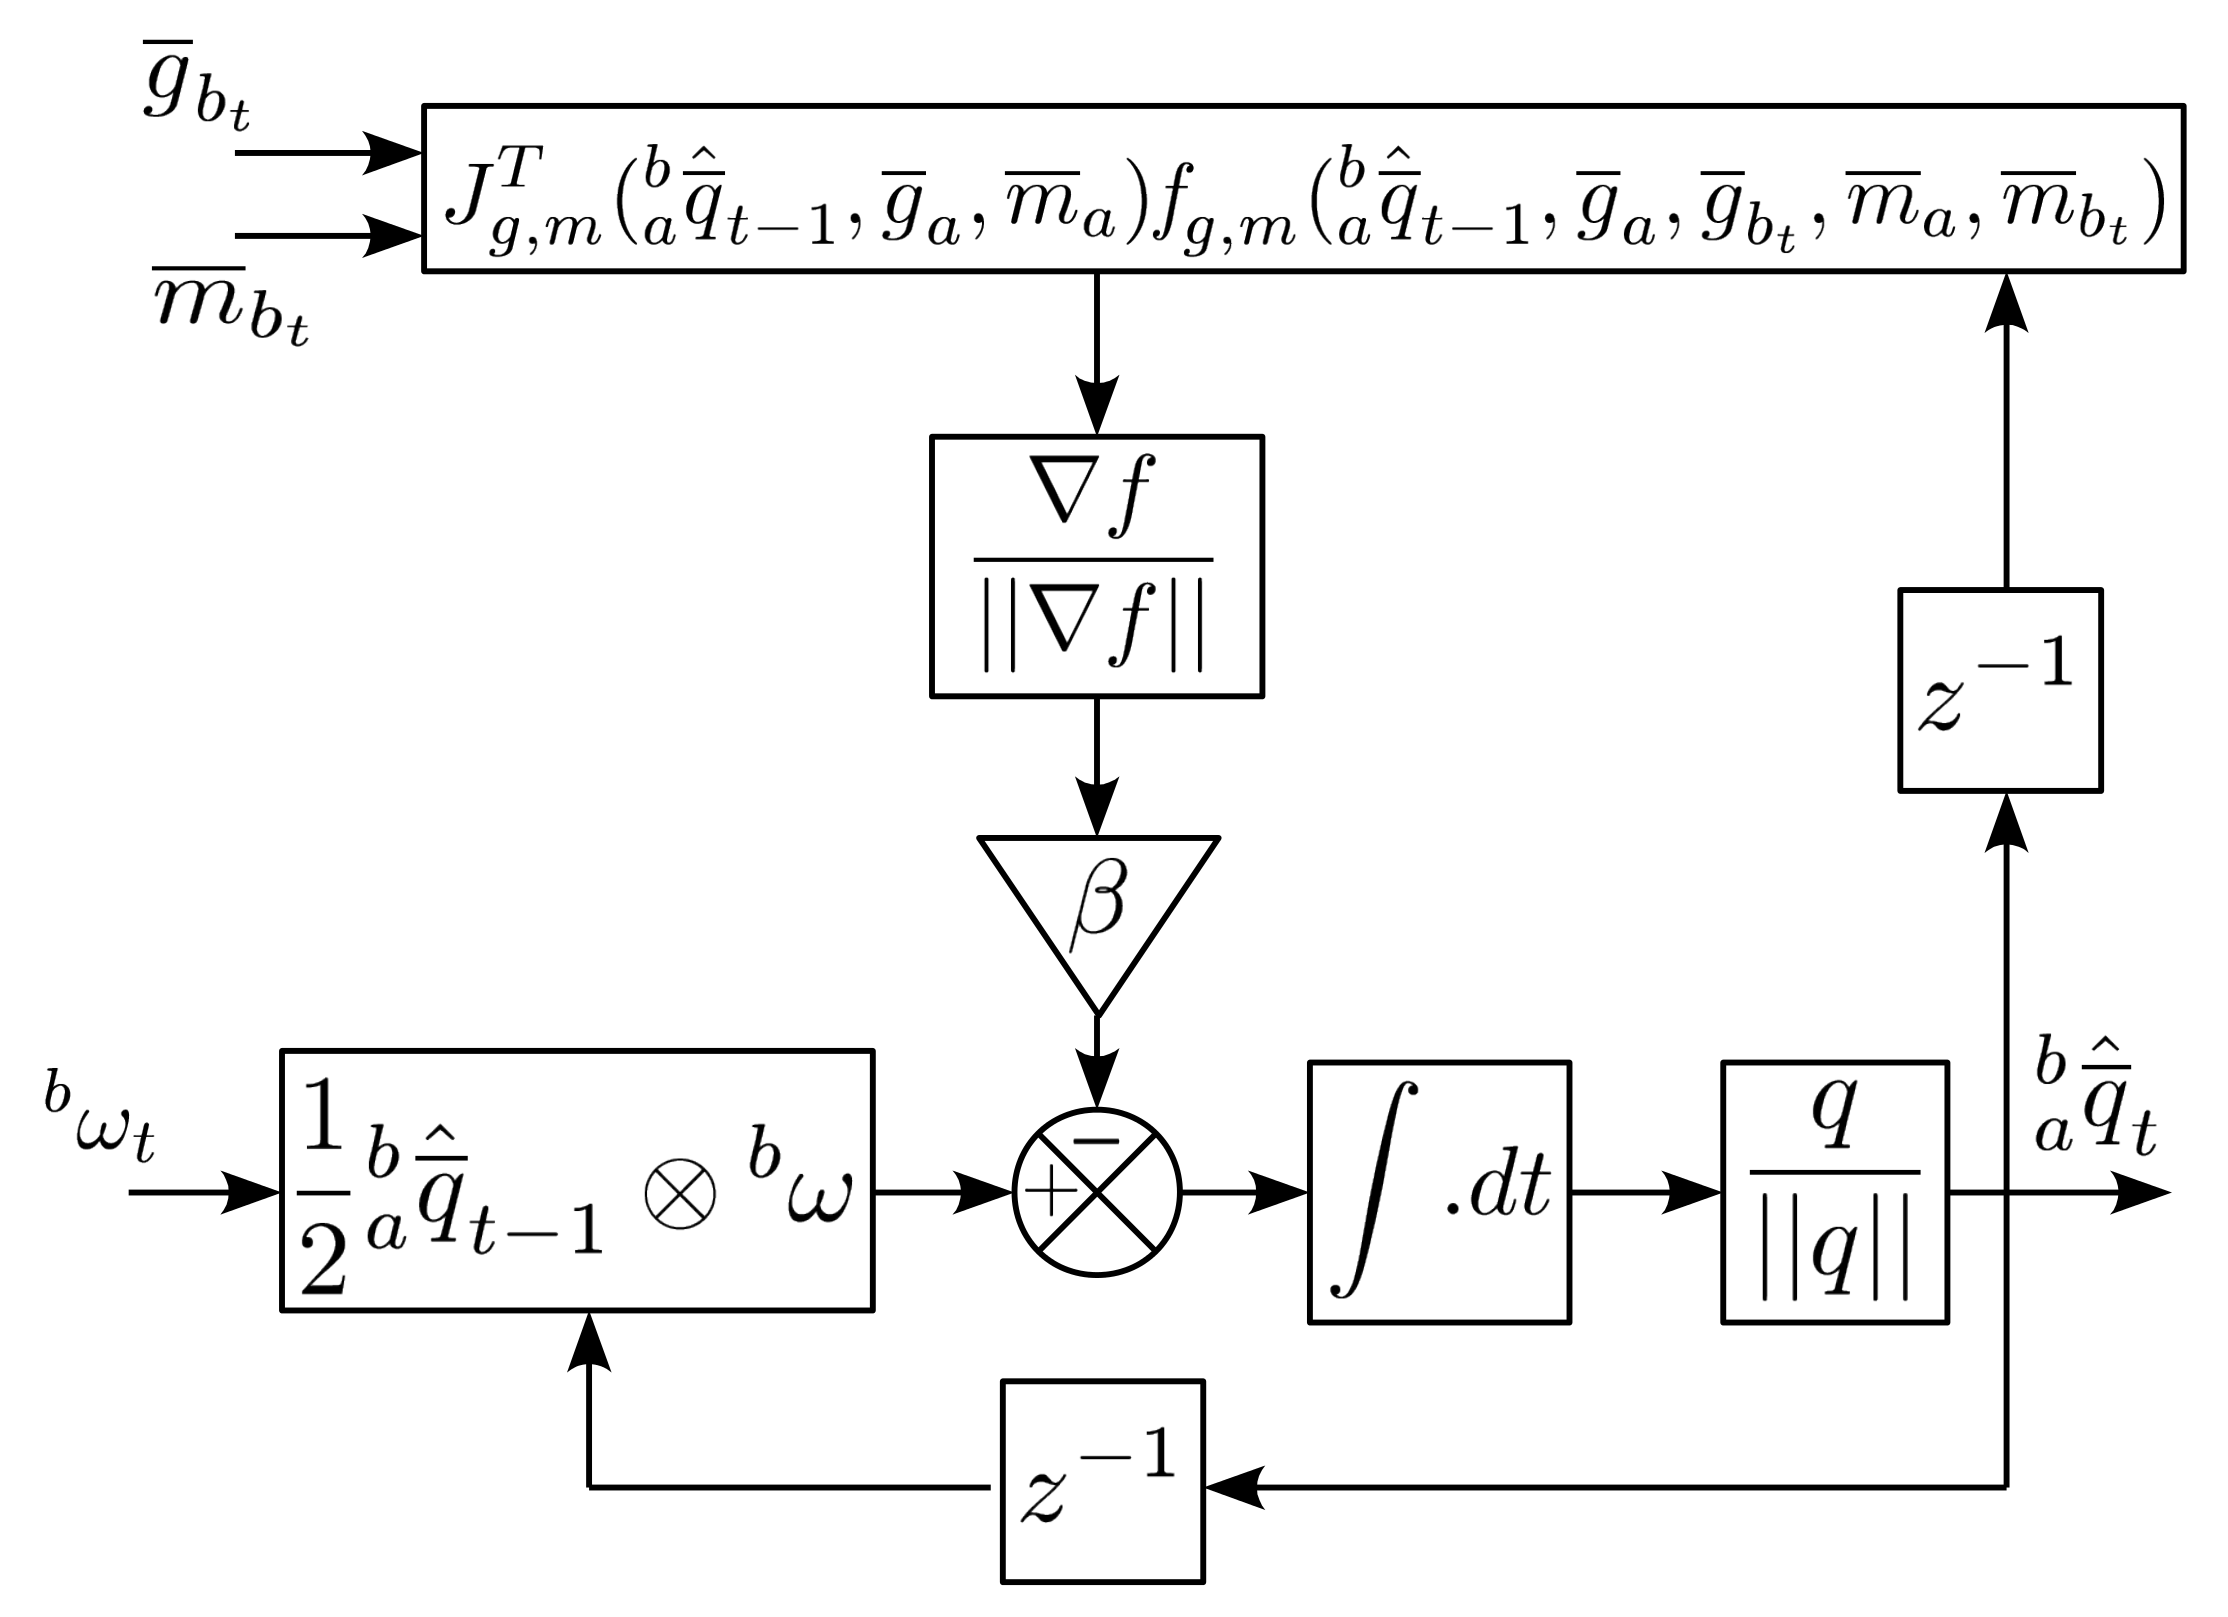
\includegraphics[scale=0.45]{Madgwick_Block_Diagram}
\caption{Block diagram of the Madgwick passive complementary filter}
\label{BlockDiagram} 
\end{figure}

\begin{algorithm}
\caption{Madgwick Discrete Filter at $n^{th}$ step}
\begin{algorithmic}[1]
\label{MadgwickAlg}
\STATE Reading the current values of the accelerometers ($g_{b_n}$), magnetometers ($m_{b_n}$) and gyro rates ($\Omega_{b_n}$) in the local IMU frame $\{B\}$
\STATE Normalizing gravity and magnetic field vector read from IMU $\overline{g}_{b_n} = \frac{g_{b_n}}{\vert \vert g_{b_n} \vert \vert}$, $\overline{m}_{b_n} \frac{m_{b_n}}{\vert \vert m_{b_n} \vert \vert}$
\STATE Computing the objective function value $f_{g,m}({^b_a\hat{\overline{q}}_{n-1}},\overline{g}_a,\overline{g}_{b_n},\overline{m}_a,\overline{m}_{b_n})$ using equations (\ref{eq4_12}) and (\ref{eq4_14})
\STATE Computing the transpose of the Jacobian of the objective function $J^T_{g,m}(^b_a\hat{\overline{q}}_{n-1},\overline{g_a},\overline{m}_a)$ using equations (\ref{eq4_13}) and (\ref{eq4_17})
\STATE Computing the correction terms $c_n =  \beta \frac{\nabla f}{\vert \vert \nabla f \vert \vert}$ using equation (\ref{eq4_16})
\STATE Computing the orientation quaternion time variation $^b_a \hat{q}_{d_n} =  (\frac{1}{2} {^b_a\hat{\overline{q}}_{n-1}} \otimes \Omega_{b_n}) - c_n$
\STATE Computing the new orientation quaternion estimation given by its previouly one and its current time variation $^b_a \hat{q}_n = ^b_a\hat{\overline{q}}_{n-1} + ^b_a \hat{q}_{d_n} \Delta t$
\STATE Normalizing the new estimated quarternion $^b_a \hat{\overline{q}}_n = \frac{^b_a \hat{q}_n}{\vert \vert ^b_a \hat{q}_n \vert \vert}$ 
\end{algorithmic}
\end{algorithm}


\noindent $\blacktriangleright$  \textbf{Hardware} \\ 
\newline

In this section the sensors will be described and how these was managed and used in the application . The information about acceleration, angular rotation velocity and  magnetic field can be obtained by an IMU (Inertial Measurements Unit).  The low power, light weight and potential for low cost manufacture of these units opens up a wide range of solution. The  purpose is to constrain rigidly one device on each phalanges of the fingers, more two  on the palm of the hand.  Although the size of a generic IMU is very small, the selection  was accurate to permit the correct assembly on the hand. Thus an Invensence product has been chosen, MPU-9250.  \\
\newline

\noindent $\bullet$ \textbf{MPU-9250}

\noindent The MPU-9250 is a System in Package (SiP) that combines two chip: the MPU-6500 (used for the paper published in ICRA2015), wich contains a 3-axis gyroscope, a 3-axis accelerometer, and an onboard Digital Motion Processor (DMP); and AK8963, the market leading 3-axis digital compass.  
\begin{figure}[h]
\centering
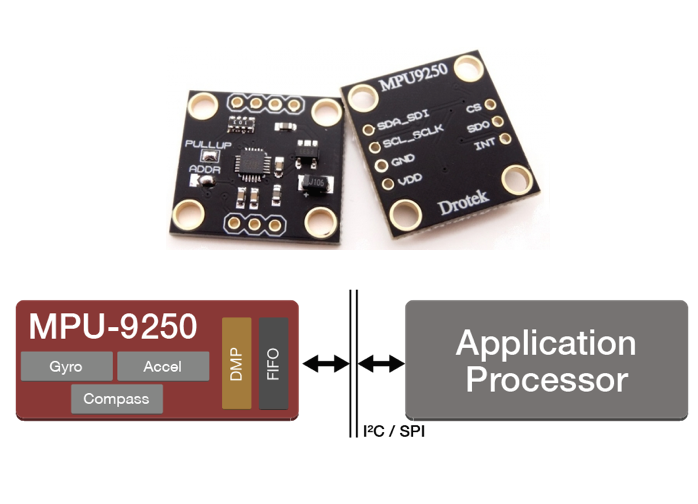
\includegraphics[scale=0.35]{mpu9250.png}
\caption{MPU-9250}
\label{fig:mpu9250}
\end{figure}

\begin{itemize}
\item[$\cdot$] \textit{Accelerometer}: the MPU-9250's accelerometers use separate proof masses for each axis. Acceleration along a particular axis induces displacement on the corresponding proof mass, and capacitive sensors detect the displacement differentially. The 3-analog informations are digitized using individual on-chip 16-bit Analog-to-Digital Converers(ADCs) to sample each axis;

 \item[$\cdot$] \textit{Gyroscope}: three indipendet vibratory rate gyroscopes are in the MPU-9250, wich detect rotation about the X, Y and Z axes. When the gyroscope are rotated about any of sense axes, the Coriolis Effect causes a ibration that is detected by a capacitive pickoff. The resulting signal is amplified, demodulated and filtered to produce a voltage that is proportional to the angular rate. This voltage pass thorugh a ADC providing digital outputs.

 \item[$\cdot$] \textit{Magnetometer}: the 3-axis magnetometer uses higly sensitive Hall sensor technology. It detects terrestrial magnetism in the X, Y and Z axes. As the other, each ADC has 16-bit resolution. 
\end{itemize}


\noindent The MPU-9250's technical features are summarized in the table \ref{tab:mpu}.
\begin{table}[tb]\footnotesize
\caption{MPU-9250 features}
\centering
\label{tab:mpu}
\begin{tabular}{l | c | l}
\textbf{Part} & \textbf{Unit} &  \\ \hline \hline
Gyro Full Scale Range & (deg/sec) &  $\begin{array}{l}   \pm 250 \\  \pm 500  \\ \pm 1000 \\ \pm \textbf{2000} \end{array}$  \\   
\rowcolor [gray]{.8}  \text{Gyro Rate Noise} &  (\text{dps}/$\sqrt{\text{Hz}}$)  & $\begin{array}{l}   0.01 \end{array}$  \\ 
\text{Accel Full Scale Range} & (\text{g}) & $\begin{array}{l}   \pm 2 \\  \pm 4 \\  \pm \textbf{8} \\ \pm 16 \end{array}$ \\ 
\rowcolor [gray]{.8} \text{Compass Full Scale Range} &($\mu\text{T}$) & $\begin{array}{l}   \pm \textbf{4800} \end{array} $\\ 
\text{Digital Output} &  & $\begin{array}{l} \text{I}^2\text{C} \\ \textbf{SPI}   \end{array} $ \\  
\rowcolor [gray]{.8} \text{Logic Supply Voltage } & (\text{V}) & $\begin{array}{l} 1.7\text{V}\text{to}\text{VDD} \\ \textbf{VDD}   \end{array} $\\ 
\text{Package Size} & (\text{mm}) & $\begin{array}{l} 3\text{x}3\text{x}1   \end{array}$ 
\end{tabular}
\end{table}


The output data from  axes sensors can be read,  in digital way, from a 8-bit  register of the device.  Each axis sensor presents two registers,   up  and  low register. Thus a complete information from a specific sensor, e.g. the accelerometer, occupies 32-bit. 

The figure \ref{fig:axes} shows the orientation of the axes of sensitivity and the polarity of rotation.
\begin{figure}[h]
\centering
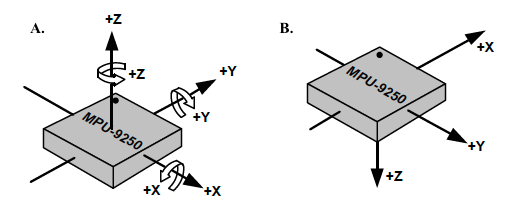
\includegraphics[scale=0.5]{axes_orientation.png}
\caption{A. accelerometer and gyro orientation axes  B. magnetometer oreintation axes}
\label{fig:axes}
\end{figure}

The necessary IMU to compute the complete posture of the hand are 17, 15 applied on each phalanges and 2 on the palm of the  hand. 
In this way the communication and data sending to a processing unit becomes a  crucial aspect. In the MPU-9250 it is possible to select two different type of communication, I$^2$C (Inter Integreted Circuit) or SPI (Serial Peripheral Interface). The I$^2$C supports a frequency of 400Hz while the SPI  1Mhz. The advantage to select the SPI way not only allows to send  data faster but 
also gives the possibility to manage more IMUs in a single communication bus, figure \ref{fig:spi}.

SPI is a 4-wire synchronous serial interface that uses two control lines and two data lines. The MPU-9250 alway operates as a Slave device during standard Master-Slave SPI operation, so the bus is made up of 4 communication line:
\begin{itemize}
\item[-] SCLK, clock;
\item[-] MOSI, master-output slave-input;
\item[-] MISO, master-input slave-output;
\item[-] SS,   slave select.
\end{itemize}

\noindent With respect to the Master, the SCLK, the MISO and the MOSI are shared among the Slaves devices. Each SPI slave devices requires its own SS line from the master. SS goes low, \textit(active) when the transmission start and goes back high \textit(inactive) at the end. Only one SS line is active at a time, ensuring that only one slave is selected at any given time.   
\begin{figure}[h]
\centering
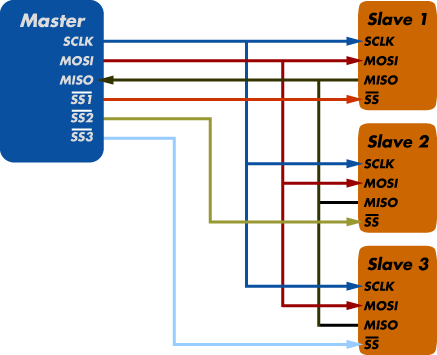
\includegraphics[scale=0.4]{spi.png}
\caption{Scheme of SPI communication}
\label{fig:spi}
\end{figure}


Usually the master is a microcontroller  or any processing unit that support SPI communication. To manage all 17 slave devices,  it is necessary a microcontroller with sufficient number of pins.   The microcontroller must be able not only to read the correct data from the IMUs but also it must send  data packages to the PC, in which the Magdwick Filter is implemented.   \\
\newline

\noindent $\bullet$ \textbf{PSoC 5LP} \textsuperscript \textregistered

\noindent The processing unit used was \textit{PSoC 5LP} developed by  Cypress Semiconductor. PSoC is a low power  ARM \textsuperscript \textregistered Cortex - M3 based programmable system on chip devices offering unmatched high-precision analog and the flexibility to design custom system solutions. When combined with the free PSoC software development tools (PSoC Creatortm and
PSoC Programmer) from Cypress, this module is more than sufficient for creating anything from basic microcontroller with embedded analog and digital functions to a highly complex system controller. Both the hardware system architecture and the software are supported by the PSoC
software tools. 
The PSoC integrated circuit is composed of a core, configurable analog and digital blocks, and programmable routing and interconnect. The configurable blocks in a PSoC are the biggest different from other microcontrollers, for this reason can be associated to the FPGA microcontroller family (Field-Programmable Gate Array). 
\begin{figure}[h]
\centering
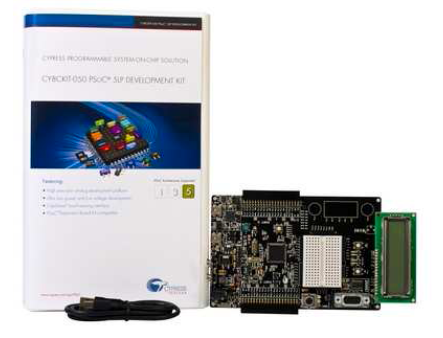
\includegraphics[scale=0.5]{psoc.png}
\caption{PSoC 5LP}
\label{fig:psoc}
\end{figure}

By using configurable analog and digital blocks, it is possible to  create and change mixed-signal embedded applications. These blocks are designed by PSoC-Creator, an Integreted Design Environment (IDE).  
The development of the PSoC 5LP  and PSoC-Creator has permitted to managed  the IMUs easily. 

The PSoC5 was exploited to read data from the slave devices allowing a SPI communication. The SPI bus could be only one, but were preferred three separated bus to have greater control on the hardware system. 

The informations from accelerometers, gyros and magnetometer were stored in the  memory of the PSoC5 ready to be sent to the PC.  The PSoC5 has a dual-channel USB interface to the host PC. Channel A of the highspeed USB interface is connected to the PSoC 5 in FIFO parallel mode to allow for the fastest possible transfers between the USB host and the PSoC 5. Channel B of the high-speed USB interface is connected to the PSoC 5 in serial mode to allow for UART communication between the host PC and the PSoC5. Using channel B USB, the PsoC can be read to the PC how a COM port, but to use this port presents an important disadvantage, the data-set can not sent if it is larger than 64 byte. For this reason another strategy was implemented. \\
\newline

\noindent $\bullet$ \textbf{Serial communication}

The communication between PSocC5 and PC was created exploiting the serial adapter 990 004. It is optimum to connect microcontroller and locig circuit to a PC. The heart of the integrated is the chip FT232R distributed by FTDI the supply a tension of 3.3V, thus it possible to connect the device to another TTL peripheral o microcontroller in the range of 3.3V-5V without the problem to convert the signal RS232 to  the TTL. The size of the circuit are very small, 25x18 mm and
\begin{figure}[h]
\centering
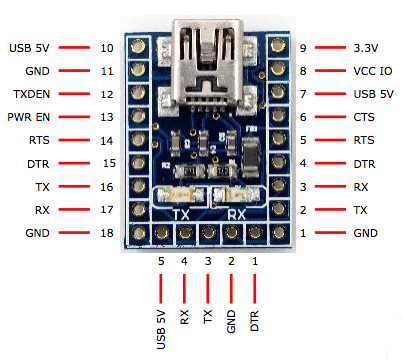
\includegraphics[scale=0.3]{usb_serial.png}
\caption{Serial adapter}
\label{fig:serial_adapter}
\end{figure}
two led visualize  input-output data of serial port, useful to continually supervise data stream escaping possible software/hardware problems. The device is USB 2.0 compatible and it permits all velocity to 1Mb. 

\begin{figure}[h]
\centering
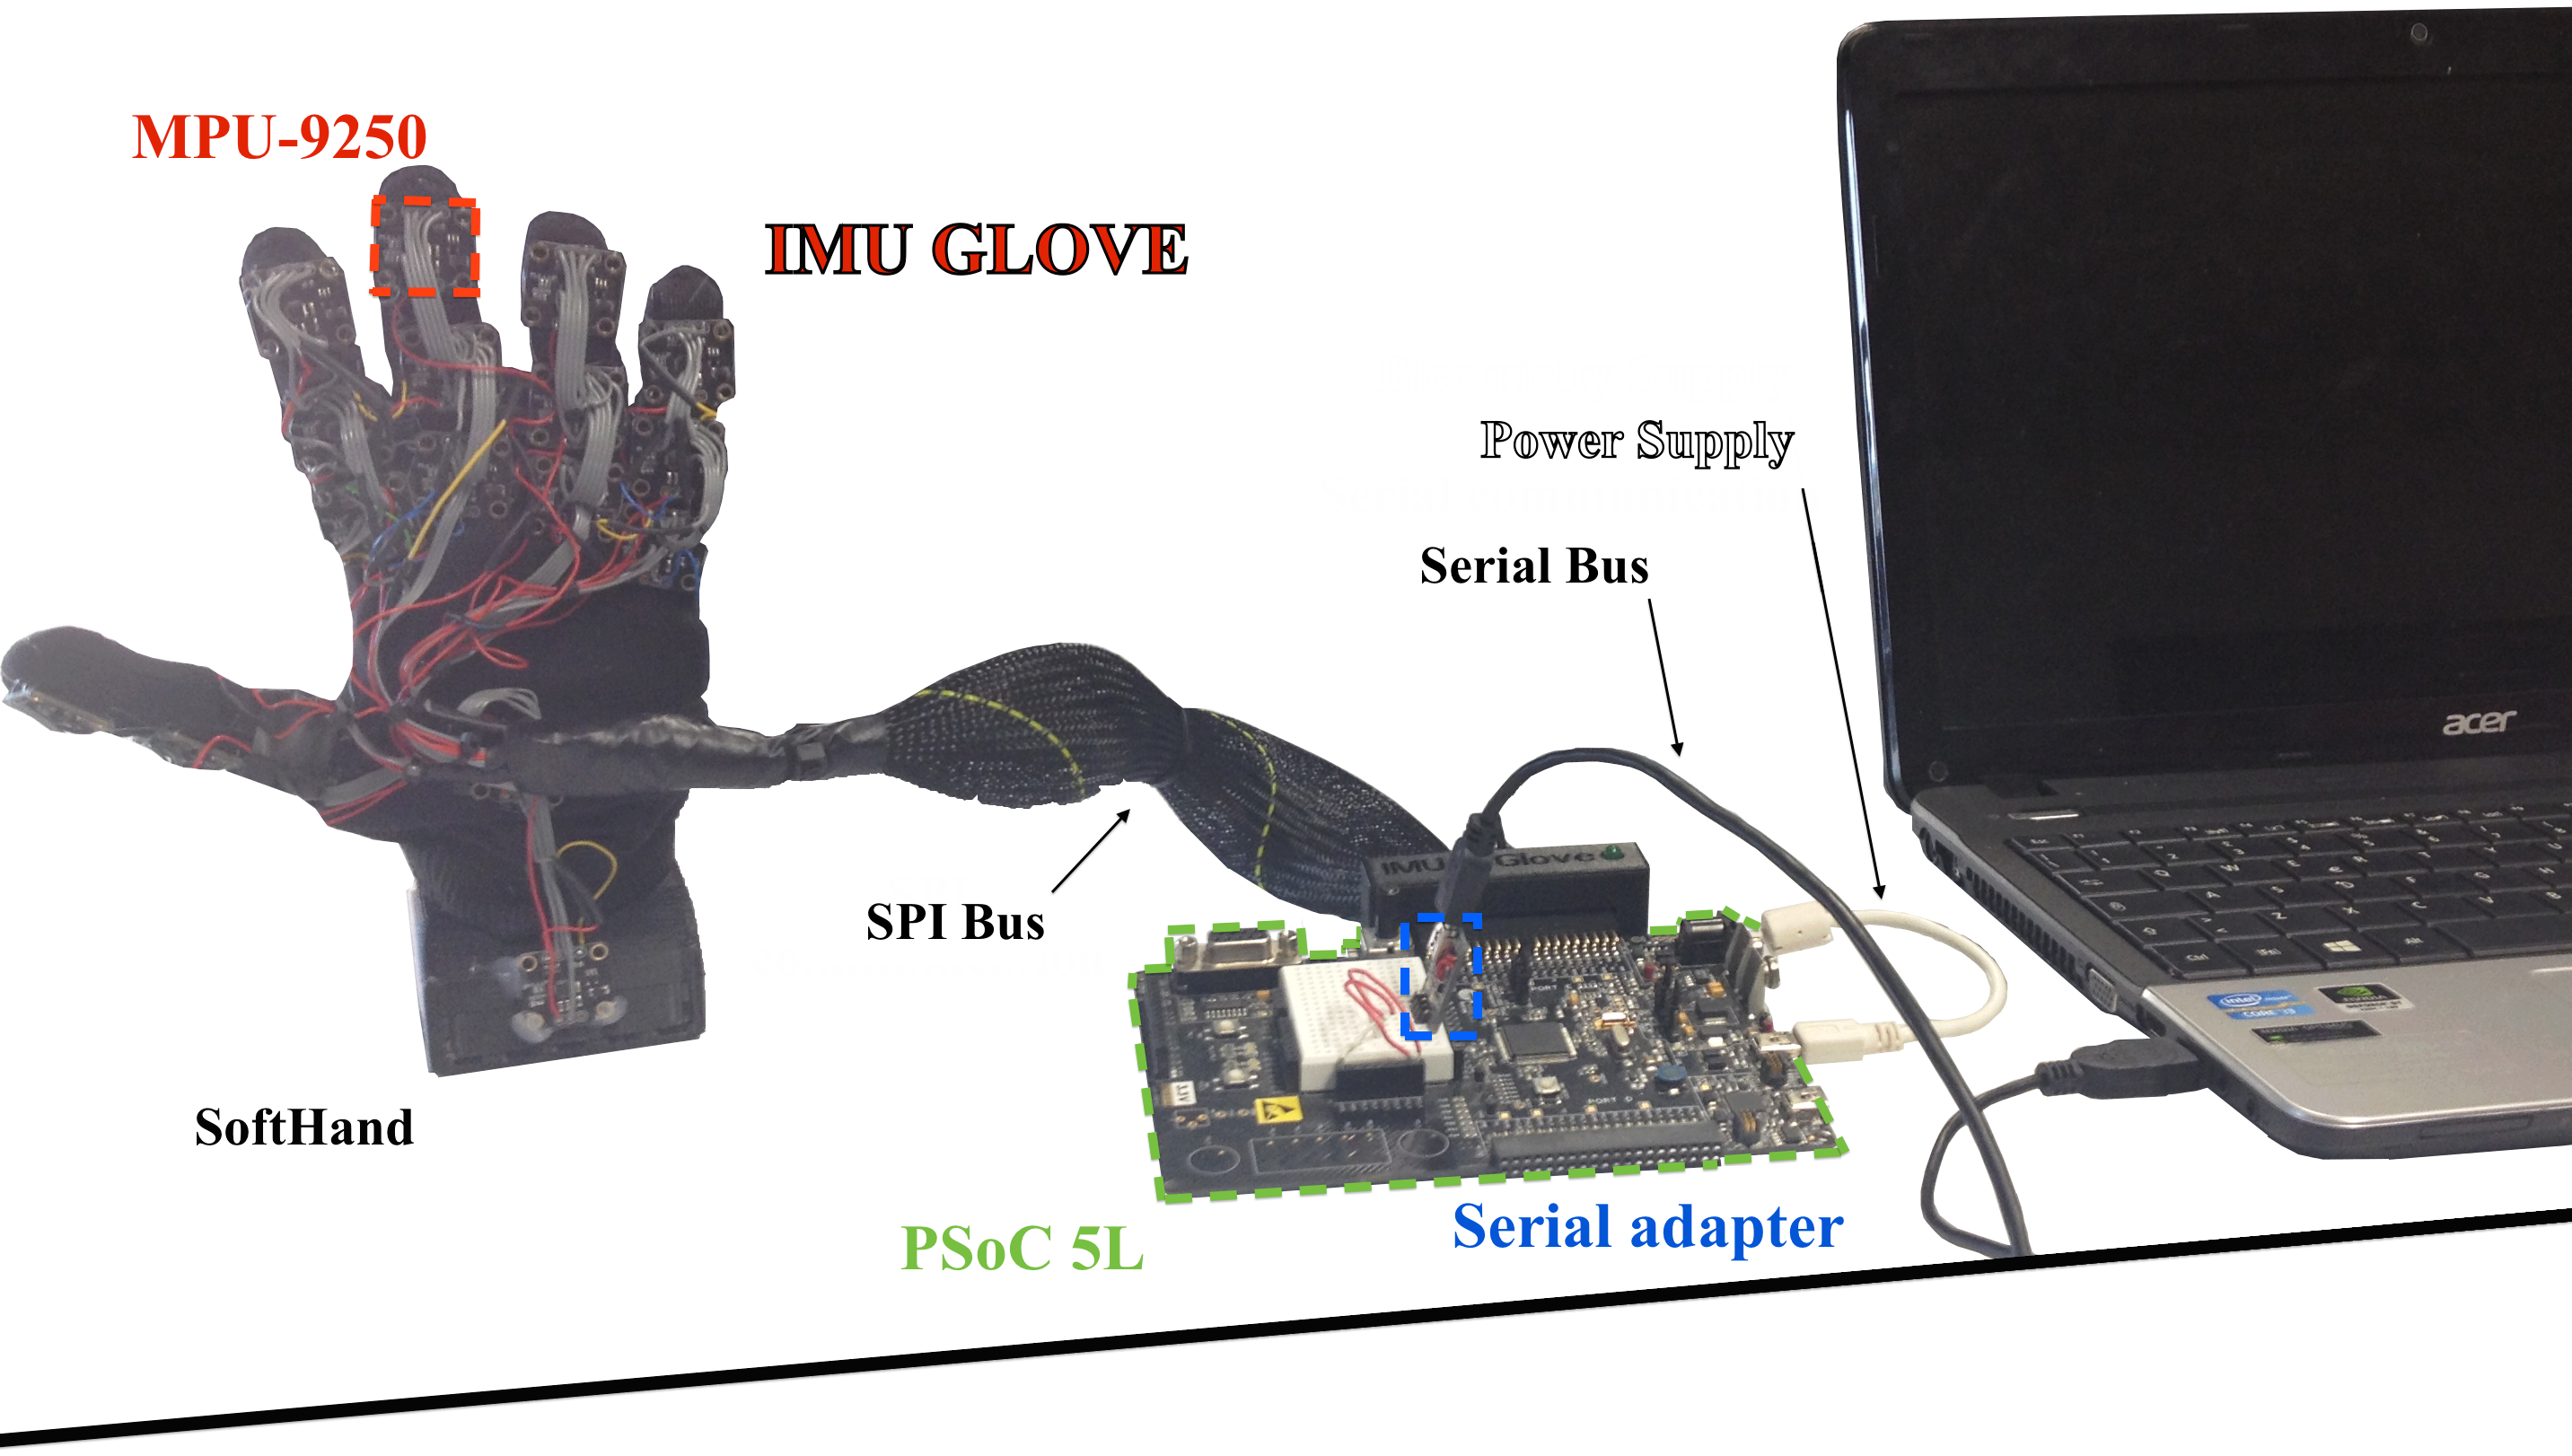
\includegraphics[scale=0.125]{hardware.png}
\caption{Full Hardware}
\label{fig:hardware}
\end{figure}


\noindent $\blacktriangleright$  \textbf{Code} \\ %\setlength{\headheight}{15pt}  \
\newline

The hardware described was managed in two fundamental step.  From one side there was the necessity to read IMU data and send its to computer, from the other side the sensor informations must be used to implement the algorithm for the  hand posture reconstruction.  
This was possible exploiting the PSoC5L where the \textit{Firmware} was installed and the \textit{Software} written in C++ in a Personal-Computer.

 \noindent $\bullet$ \textbf{Firmware}

 


\noindent $\bullet$ \textbf{Software}
